\section{Thermal Camera module Lepton 2.5}
\label{sec:thermalcamera}
The thermal camera module we use in this project its made by FLIR, we will go
through its techincal specification, modes of capture and communication protocol
for both video frame transfer and camera control. Information about the camera
are extracted from official documentation.
\subsection{Specification}
\label{ssec:specificationthermalcam}
Lepton is an infra-red camera system that integrates a fixed-focus lens assembly,
an $80 \times 60$ long-wave infra-red (LWIR) micro-bolometer sensor array, and
signal-processing electronics. Easy to integrate and operate, Lepton is intended
for mobile devices as well as any application requiring very small
footprint, very low power, and instant-on operation. Lepton can be operated in
its default mode or configured into other modes through a command and control
interface (CCI). The effective frame rate of the camera is only 8.6 \si{\hertz},
however for our needs this is not a problem. The camera only requires low
voltage supply and has small power consumption of around 140 \si{\milli\watt}.
\begin{figure}[!htb]
    \centering
    \subfloat[][\emph{with and without socket}.\label{fig:camerarender1}]
        {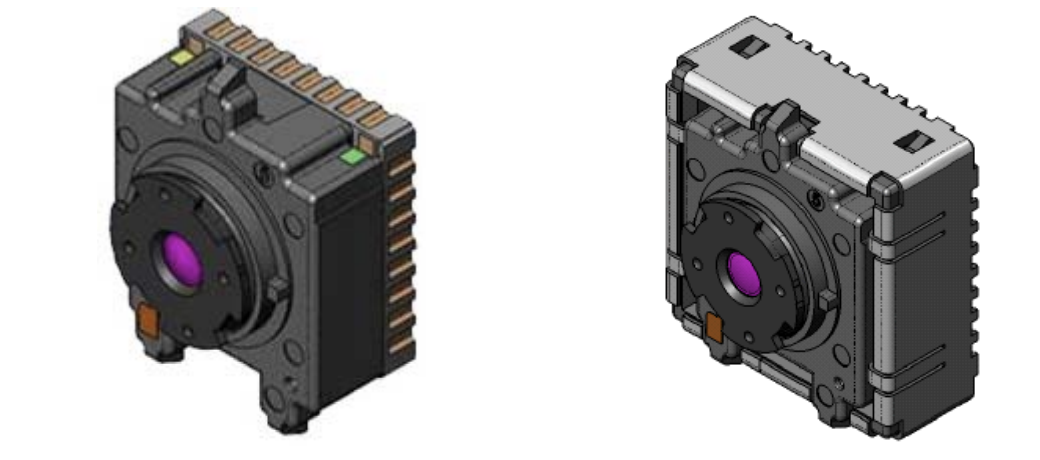
\includegraphics[width=0.5\textwidth]{leptoncamera.png}} \quad
    \subfloat[][\emph{Pinout Diagram}.\label{subfig:Pinout Diagram}]
        {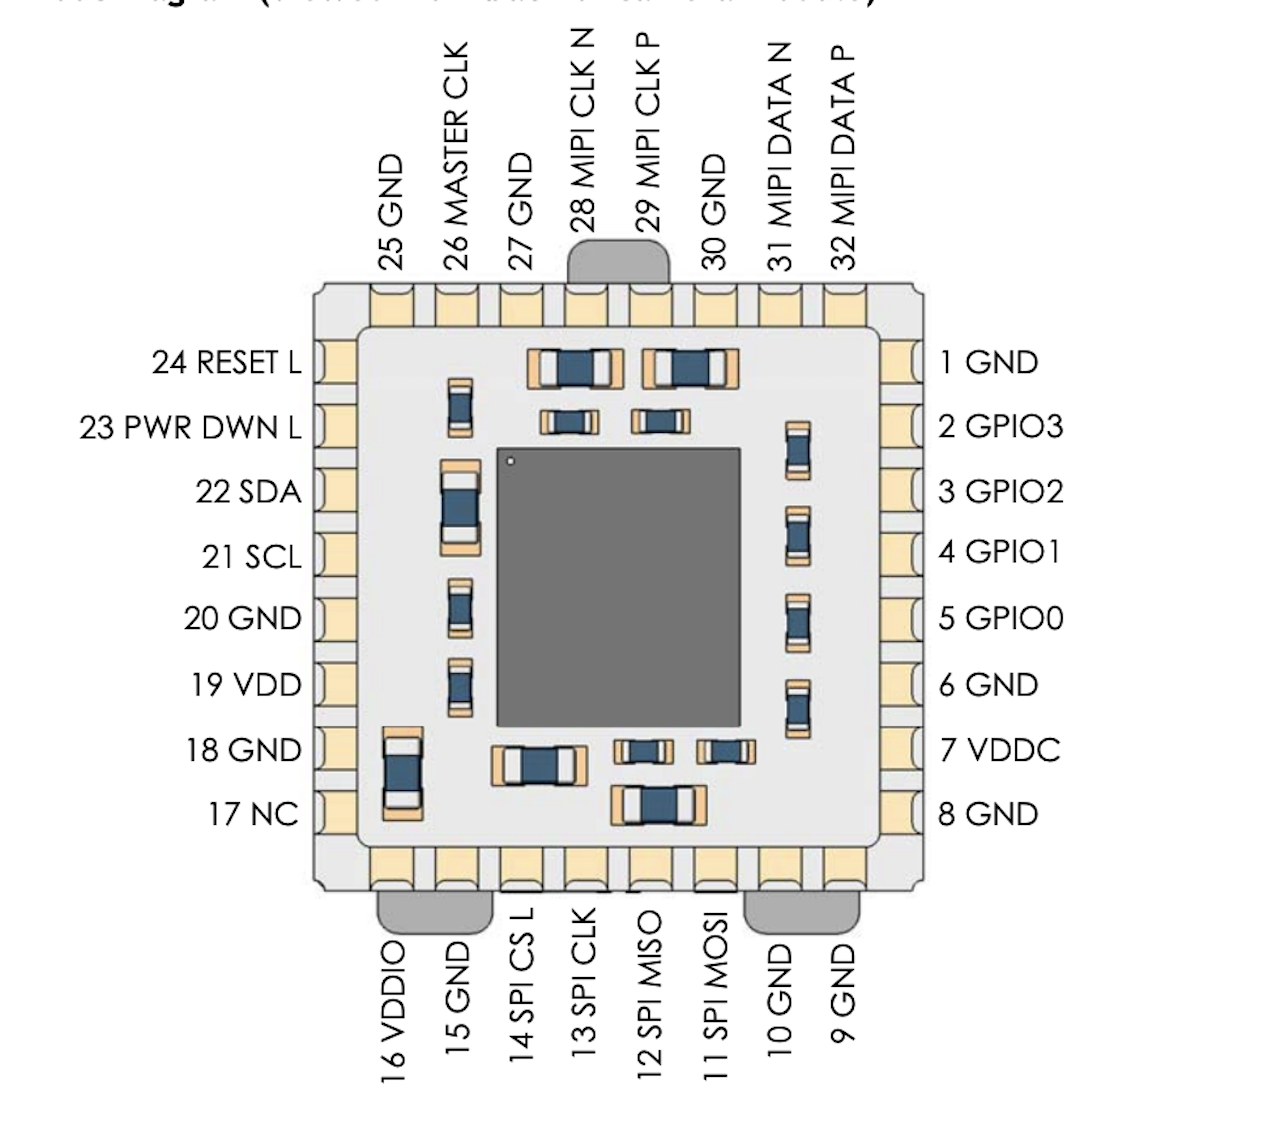
\includegraphics[width=.30\textwidth]{pinout.png}}
    \caption{Lepton Camera}
    \label{fig:camerarender}
\end{figure}
%
\begin{table}[htb]
    \centering
    \caption{Key Specifications}
    \label{tab:thcamspecifications}
    \begin{tabular}{l c c}
        \hline
                                                            &   FLIR Lepton 2.5 	&          	\\
        \hline
        \rowcolor{aliceblue!85} Resolution (h x w)	       	&   80 $\times$ 60  	&	pixels	\\
        Spectral Range	                                    	&   8  to 14        	&	\si{\micro\meter}	\\
        \rowcolor{aliceblue!85} Horizontal Field of View		&   51              	&   \si{\degree}			\\
        Thermal Sensitivity	                                	&   < 50            	&   \si{\milli\kelvin}	\\
        \rowcolor{aliceblue!85} Frame Rate	                	&   < 9             	&   \si{\hertz} 			\\
        Control Interface	                                	&   I$^{2}$C        	&               			\\
        \rowcolor{aliceblue!85} Video Interface	            	&   SPI             	&               			\\
        Promised Time to Image	                            	&   < 0.5           	&   \si{\second}    		\\
        \rowcolor{aliceblue!85} Integral Shutter		    		&   yes             	&   			\\
        Radiometry	                                        	&   14-bit pixel value  	&       \\
        \rowcolor{aliceblue!85} Operating Power             	&	$\sim$150       	&   \si{\milli\watt} 	\\
        \hline
\end{tabular}
\end{table}
%
\linebreak See table \ref{tab:thcamspecifications} for more specifications. For better
manipulation with the camera module we use a breakout board (figure \ref{fig:breakoutboard}) with a
housing for the Lepton camera module. The breakout board provides better
physical accessibility, improves heat dissipation and increases input voltage
supply range to 3--5 \si{\volt}, as it has its own regulated power supply. This
power supply provides the camera module with three necessary voltages: 1.2, 2.8
and 2.5--3.1 \si{\volt}. The breakout board also supplies the camera with master
clock signal.\cite{breakoutboard}
%
\begin{figure}[!htb]
    \centering
    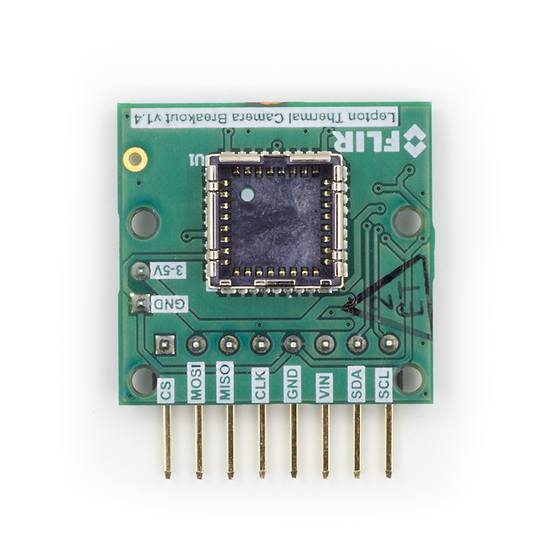
\includegraphics[width=0.50\textwidth]{Lepton_Breakout_Board_-_s_550x825.png}
    \caption{Breakout board.}
    \label{fig:breakoutboard}
 \end{figure}
\linebreak The camera uses two interfaces for communication:
\begin{itemize}
    \item SPI for transferring video frames from the camera to a SPI master
device.
    \item I$^{2}$C for receiving control commands from the I$^{2}$C master
device.
\end{itemize}
%
\begin{figure}[htb]
    \centering
    \resizebox{0.8\textwidth}{!}{
\begin{tikzpicture}
    \draw[help lines] (0,0) grid (20, 20);
%     \draw (0,0) rectangle (10,20);
% \draw[fill=cyan!50] (1,1) rectangle (7,3)   node {Camera Supply Inputs};
% \draw[fill=cyan!50] (1,3) rectangle (7,6)   node {Camera Shut Down};
% \draw[fill=cyan] (1,6) rectangle (7,11) node {Camera Reset};
% \draw[fill=cyan!50] (1,11) rectangle (7,13) node {Camera Clock Gneration};
% \draw[fill=cyan!50] (1,13) rectangle (7,15) node {Camera };
% \draw[fill=cyan!50] (1,15) rectangle (7,17) node {Camera };
% \draw[fill=cyan!50] (1,17) rectangle (7,19) node {Camera };
% \draw[fill=cyan!50] (1,1) rectangle (,);
% \draw[fill=cyan!50] (1,1) rectangle (,);
% \draw[fill=cyan!50] (1,1) rectangle (,);
% \draw[fill=cyan!50] (1,1) rectangle (,);
% \draw[fill=cyan!50] (1,1) rectangle (,);
% \draw[fill=cyan!50] (1,1) rectangle (,);
% \draw[fill=cyan!50] (1,1) rectangle (,);
% \draw[fill=cyan!50] (1,1) rectangle (,);
% \draw[fill=cyan!50] (1,1) rectangle (,);
% \draw[fill=cyan!50] (1,1) rectangle (,);
% \draw[fill=cyan!50] (1,1) rectangle (,);
% \draw[fill=cyan!50] (1,1) rectangle (,);
% \draw[fill=cyan!50] (1,1) rectangle (,);
% \draw[fill=cyan!50] (1,1) rectangle (,);
% \draw[fill=cyan!50] (1,1) rectangle (,);








\end{tikzpicture}
}
    \caption{my figure drawn in tikz}
    \label{fig:myfigure}
\end{figure}
%
\subsection{System Architecture}
\label{ssec:leptonarchitecture}
The lens assembly focuses infrared radiation from the scene onto an $80 \times 60$ array
of thermal detectors with 17-micron pitch. Each detector element is a
vanadium-oxide (VOx) microbolometer whose temperature fluctuates in response to
incident flux. The change in temperature causes a proportional change in each
microbolometer’s resistance. VOx provides a high temperature coefficient of
resistance (TCR) and low $1/f$ noise, resulting in excellent thermal sensitivity
and stable uniformity. The microbolometer array is grown monolithically on top
of a readout integrated circuit (ROIC) to comprise the complete focal plane
array (FPA). Once per frame, the ROIC senses the resistance of each detector by
applying a bias voltage and integrating the resulting current for a finite
period of time called the integration period. The serial stream from the FPA is
received by a system on a chip (SoC) device, which provides signal processing
and output formatting.
%
\subsection{video pipeline}
\label{ssec:pipeline}
The video pipeline includes non-uniformity correction (NUC), defect replacement,
spatial and temporal filtering, automatic gain correction (AGC), and
colourization.
%
%insert image video stream
%
% nuc
\paragraph{The non-uniformity correction (NUC)} block applies correction
terms to ensure that the camera produces a uniform output for each pixel when
imaging a uniform thermal scene. Factory-calibrated terms are applied to
compensate for temperature effects, pixel response variations, and
lens-illumination roll-off. To compensate for temporal drift, the NUC block also
applies an offset term that can be periodically updated at runtime via a process
called flat-field correction (FFC). The FFC process is further described in FFC
States, (\ref{ssec:FFCstates}).
%
%7.2 Defect Replacement
\paragraph{The defect-replacement} block substitutes for any pixels identified
as defective during factory calibration or during runtime. The replacement
algorithm assesses the values of neighboring pixels and calculates an optimum
replacement value. The typical number of defective pixels is $\leq 1$.
%
\paragraph{Temporal Filtering} the image pipeline includes a number of
sophisticated image filters designed to enhance signal-to-noise ratio (SNR) by
eliminating temporal noise and residual non-uniformity. The filtering suite
includes a scene-based non-uniformity correction (SBNUC) algorithm which relies
on motion within the scene to isolate fixed pattern noise (FPN) from image
content.
%
\paragraph{The AGC algorithm} for converting the full-resolution (14-bit)
thermal image into a contrast-enhanced image suitable for display is a
histogram-based non-linear mapping function. See (\ref{ssec:AGCModes}).
%
\paragraph{The colorize block} takes the contrast-enhanced thermal image as
input and generates a 24-bit RGB color output.
%
\subsection{Power States}
\label{ssec:powerstate}
Lepton currently provides five power states. As depicted in the state diagram
shown in Figure 6, most of the transitions among the power states are the result
of explicit action from the host. The automatic transition to and from the
overtemp state is an exception. In the figure, transitions that require specific
host-side action are shown in bold. Automatic transitions are not bolded.
%
\begin{itemize}
    \item Off: When no voltage is applied, Lepton is in the off
state. In the off state, no camera functions are available.
    \item Uninitialized:
In the uninitialized state, all voltage forms are applied, but Lepton has not
yet been booted and is in an indeterminate state. It is not recommended to leave
Lepton in this state as power is not optimized; it should instead be booted to
the on-state (and then transitioned back to standby if imaging is not required).
    \item On: In the on state, all functions and interfaces are fully available.
    \item Standby: In the standby state, all voltage forms are applied, but power
consumption is approximately 4 \si{\milli\watt}. In the standby state, no
functions are available, but it is possible to transition to the on state via
the start-up sequence defined in Figure 7 on page 16. The shutdown sequence
shown in Figure 7 on page 16 is the recommended transition back to the standby
state. It is also possible to transition between standby and on states via
software commands, as further defined in the software IDD.
    \item Overtemp: The
overtemp state is automatically entered when the Lepton senses that its
temperature has exceeded approximately $80$ \si{\celsius}. Upon entering the
overtemp state, Lepton enables a ``\emph{shutdown imminent}" status bit in the
telemetry line and starts a $10$ \si{\second} counter. If the temperature of the
Lepton falls below $80$ \si{\celsius} before the counter times out, the
``\emph{shutdown imminent}" bit is cleared and the system transitions back to
the on state. If the counter does time out, Lepton automatically transitions to
the standby state.
\end{itemize}
%
\subsection{FFC States}
\label{ssec:FFCstates}
Lepton is factory calibrated to produce an output image that is highly uniform,
such as shown in Figure \ref{subfig:Highly uniform image}, when viewing a
uniform-temperature scene. However, drift effects over long periods of time
degrade uniformity, resulting in imagery which appears more grainy (Figure
\ref{subfig:Grainy image}) and/or blotchy (Figure \ref{subfig:Blotchy image}).
Operation over a wide temperature range (for example, powering on at $-10$
\si{\celsius} and heating to $65$ \si{\celsius}) will also have a detrimental
effect on image quality. For scenarios in which there is ample scene movement,
such as most handheld applications, Lepton is capable of automatically
compensating for drift effects using an internal algorithm called scene-based
non-uniformity correction (scene-based NUC or SBNUC). However, for use cases in
which the scene is essentially stationary, such as fixed-mount applications,
scene-based NUC is less effective. In those applications, it is recommended to
periodically perform a flat-field correction (FFC). FFC is a process whereby the
NUC terms applied by the camera's signal processing engine are automatically
recalibrated to produce the most optimal image quality. The sensor is briefly
exposed to a uniform thermal scene, and the camera updates the NUC terms to
ensure uniform output. The entire FFC process takes less than a second.
%
\begin{figure}[htb]
    \centering
    \subfloat[][\emph{Highly uniform image}.\label{subfig:Highly uniform image}]
        {
\includegraphics[width=.30\textwidth]{uniform}} \quad
    \subfloat[][\emph{Grainy image
    (high-spatial frequency noise)}.\label{subfig:Grainy image}]
        {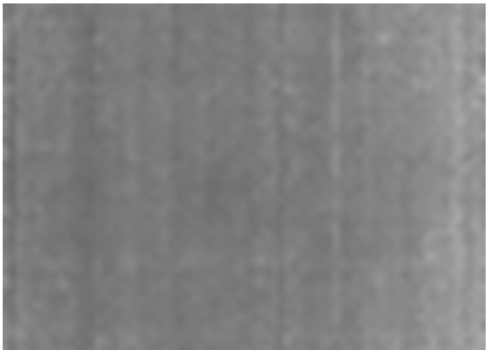
\includegraphics[width=.30\textwidth]{grainy.png}} \quad
    \subfloat[][\emph{ Blotchy image
    (low-spatial frequency noise)}.\label{subfig:Blotchy image}]
        {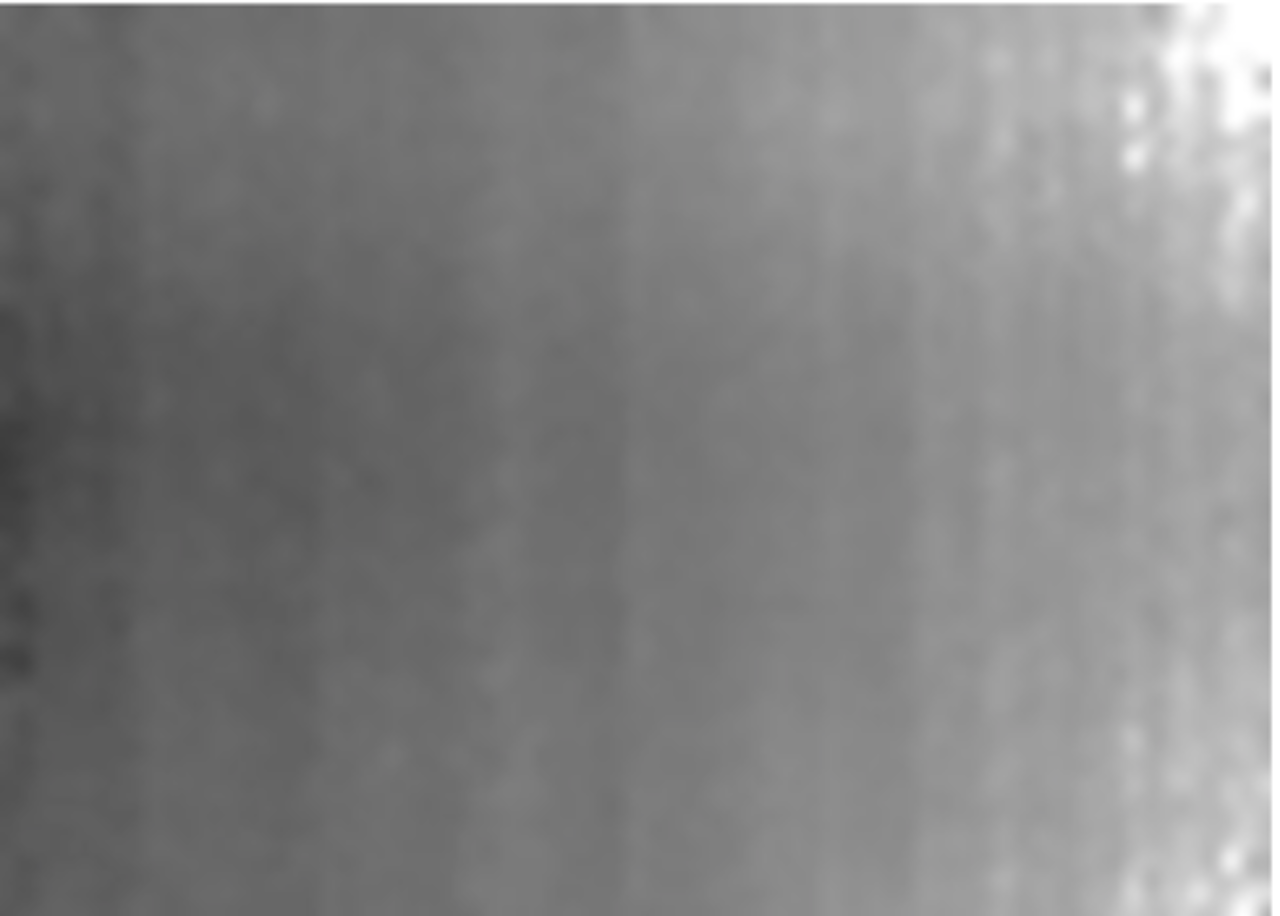
\includegraphics[width=.30\textwidth]{blotchy.png}}
    \caption{Examples of Good Uniformity, Graininess, and Blotchiness}
    \label{fig:exampleffc}
\end{figure}
%
\\The current FFC state is provided through the telemetry line. There are three
FFC states, as illustrated in Figure \ref{fig:FFC States}:
\begin{enumerate}
    \item FFC not commanded (default): In this state, Lepton applies by default a
set of factory-generated FFC terms.
    \item FFC in progress: Lepton enters this
state when FFC is commanded. The default FFC duration is nominally $23$ frames.
    \item FFC complete: Lepton automatically enters this state whenever FFC is
completed. Lepton also provides an ``FFC desired" flag in the telemetry line.
The ``FFC desired" flag is asserted at start-up, when a specified period
(default = 3 minutes) has elapsed since the last FFC, or when the sensor
temperature has changed by a specified value (default = 3 \si{\celsius}) since
the last FFC. The ``FFC desired" flag is intended to indicate to the host to
command an FFC at the next possible opportunity.
\end{enumerate}
%
\begin{figure}[htb]
    \centering
    \resizebox{0.35\textwidth}{!}{\begin{tikzpicture}
    \node (start) at (1,12) {Lepton powered on};
    \node [ellipse, fill=babyblueeyes, align=center] (notcommand) at (1,10) {FFC Not \\ Commanded};
    \node [ellipse, fill=babyblueeyes] (progress) at (1,8) {FFC In Progress};
    \node [ellipse, fill=babyblueeyes] (complete) at (1,6) {FFC Complete};
    \draw [-latex] (start) to (notcommand);
    % connections
    \path[-latex] (notcommand)  edge [bend right=50]    node[left] {\tiny{FFC Commanded}} (progress);
    \path[-latex] (progress)    edge [bend left=50]     node[right] {\tiny{FFC Complete}} (complete);
    \path[-latex] (complete)    edge [bend left=50]     node[left] {\tiny{FFC Commanded}} (progress);
\end{tikzpicture}
}
    \caption{FFC States.}
    \label{fig:FFC States}
\end{figure}
%
\subsection{AGC Modes}
\label{ssec:AGCModes}
There are two AGC modes:
\begin{itemize}
    \item AGC disabled (default)
    \item AGC enabled
\end{itemize}
AGC is a process whereby the large dynamic range of the infrared sensor is
collapsed to a range more appropriate for a display system. For Lepton, this is
a 14-bit to 8-bit conversion. In its most simplistic form, AGC can be a linear
mapping from 14-bit to 8-bit; however, a simple linear AGC is generally
incapable of providing pleasing imagery in all imaging conditions. For example,
when a scene includes both cold and hot regions (for example, a hot object in
front of a cold background as illustrated in \ref{fig:comparisionlinearAGC},
linear AGC can produce an output image in which most pixels are mapped to either
full black or full white with very little use of the gray shades (8-bit values)
in between. Because of this limitation of linear AGC, a more sophisticated
algorithm is preferred. Similar to most AGC algorithms that optimize the use of
gray shades, Lepton's is histogram-based. Essentially a histogram counts the
number of pixels in each frame that have a given 14-bit value. Figure
\ref{fig:histogram} the concept for a 3x3 pixel area.\linebreak
%
\begin{figure}[!h]
    \centering
    \resizebox{0.80\textwidth}{!}{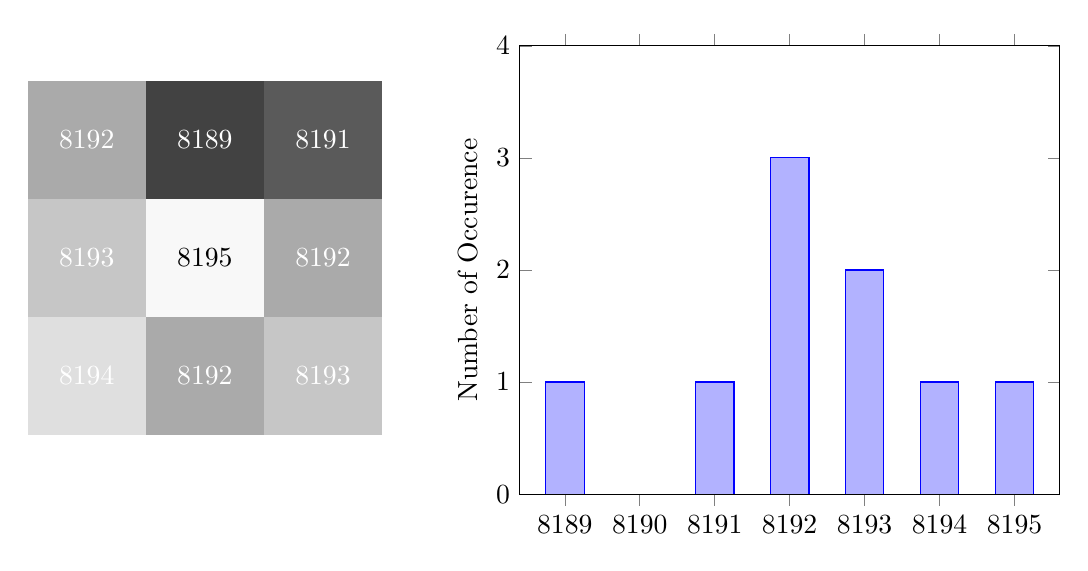
\begin{tikzpicture}
    \begin{scope}[xshift=-35mm]
        % upper row
        \node [rectangle, minimum size=15mm, fill={rgb,255:red,170; green,170; blue,170}](8192) at (1.5,4.5)   {\textcolor{white}{$8192$}};
        \node [rectangle, minimum size=15mm, fill={rgb,255:red,66; green,66; blue,66}](8189) at (3,4.5)     {\textcolor{white}{$8189$}};
        \node [rectangle, minimum size=15mm, fill={rgb,255:red,90; green,90; blue,90}](8191) at (4.5,4.5)   {\textcolor{white}{$8191$}};
        % mid row
        \node [rectangle, minimum size=15mm, fill={rgb,255:red,198; green,198; blue,198}](8193) at (1.5,3)     {\textcolor{white}{$8193$}};
        \node [rectangle, minimum size=15mm, fill={rgb,255:red,248; green,248; blue,248}](8195) at (3,3)       {\textcolor{black}{$8195$}};
        \node [rectangle, minimum size=15mm, fill={rgb,255:red,170; green,170; blue,170}](8192) at (4.5,3)     {\textcolor{white}{$8192$}};
        % lower row
        \node [rectangle, minimum size=15mm, fill={rgb,255:red,223; green,223; blue,223}](8194) at (1.5,1.5)   {\textcolor{white}{$8194$}};
        \node [rectangle, minimum size=15mm, fill={rgb,255:red,170; green,170; blue,170}](8192) at (3,1.5)     {\textcolor{white}{$8192$}};
        \node [rectangle, minimum size=15mm, fill={rgb,255:red,198; green,198; blue,198}](8193) at (4.5,1.5)   {\textcolor{white}{$8193$}};
    \end{scope}
    \begin{scope}[xshift=35mm]
        \begin{axis}[
            x tick label style={/pgf/number format/1000 sep=},
            ybar, bar width=14pt,
            ymin=0, ymax=4,
            ylabel = Number of Occurence,
            area style
        ]
    \addplot coordinates { (8189, 1) (8190, 0) (8191, 1) (8192, 3) (8193, 2) (8194, 1) (8195, 1) };
    \end{axis}
\end{scope}
\end{tikzpicture}
}
    \caption{Illustration of a Histogram for a $3 \times 3$ Pixel Area.}
    \label{fig:histogram}
\end{figure}
%
Classic histogram equalization uses the cumulative histogram as a
mapping function between 14-bit and 8-bit. The intent is to devote the most gray
shades to those portions of the input range occupied by the most pixels. For
example, an image consisting of $60 \%$ sky devotes $60 \%$ of the available
gray shades to the sky, leaving only $40 \%$ for the remainder of the image. By
comparison, linear AGC ``wastes" gray shades when there are gaps in the
histogram, whereas classic histogram equalization allocates no gray shades to
the gaps. This behavior is in principle an efficient use of the available gray
shades, but there are a few drawbacks:
\begin{itemize}
    \item The resulting contrast between an object and a much colder (or hotter)
background can be rendered poor by the fact the algorithm ``collapses" the
separation between such that the object is only one step gray shade above the
background. This phenomenon is illustrated in \ref{fig:comparisionlinearAGC}.
    \item Too much emphasis can be placed on background clutter, particularly
when a mostly isothermal background comprises a large fraction of the total
image area. This is also illustrated in \ref{fig:comparisionlinearAGC}. The
Lepton AGC algorithm is a modified version of classic histogram equalization
that mitigates these shortcomings. One such modification is a parameter called
``clip limit high". It clips the maximum population of any single bin, limiting
the influence of heavily populated bins on the mapping function. Another
parameter utilized by the Lepton algorithm is called ``clip limit low". It adds
a constant value to every non-zero bin in the histogram, resulting in additional
contrast between portions of the histogram separated by gaps. Figure
\ref{fig:comparisionlinearAGC} is an example showing the benefit of the Lepton
clip parameters.
%
\end{itemize}
\begin{figure}[!h]
    \centering
    \subfloat[][\emph{Linear AGC}.\label{subfig:linearagc}]
        {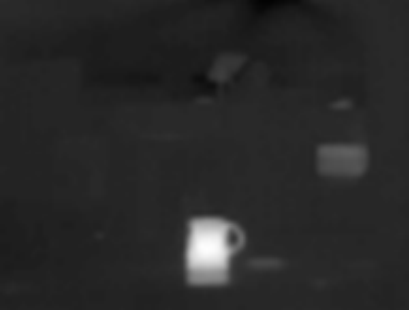
\includegraphics[width=.30\textwidth]{linearAGCa}} \quad
    \subfloat[][\emph{Classic Histogram Equalization}.\label{subfig:histrogram}]
        {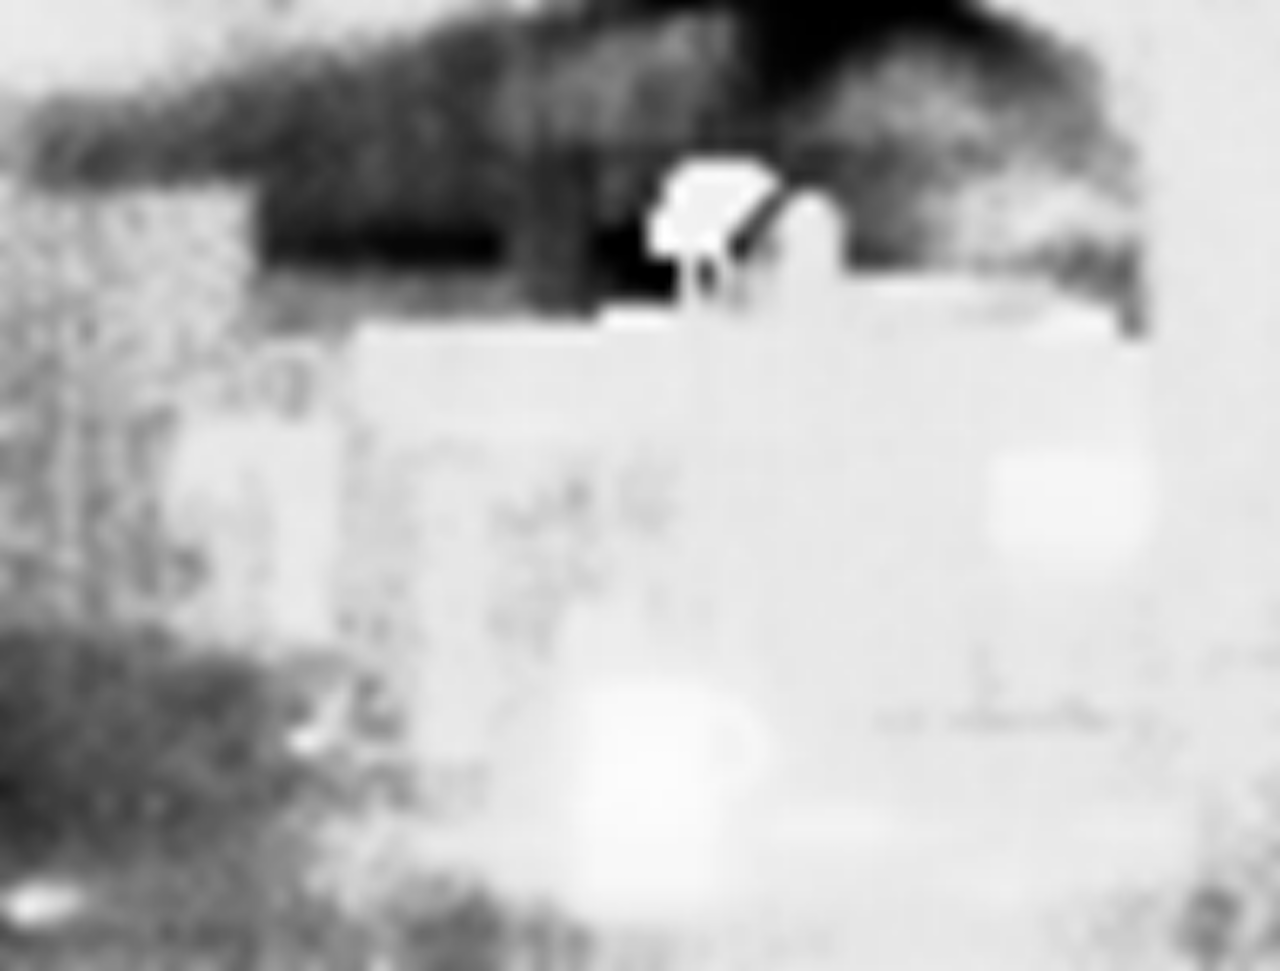
\includegraphics[width=.30\textwidth]{linearAGCb.png}} \quad
    \subfloat[][\emph{Lepton's Variant of HistogramEqualization}.\label{subfig:varianhistograms}]
        {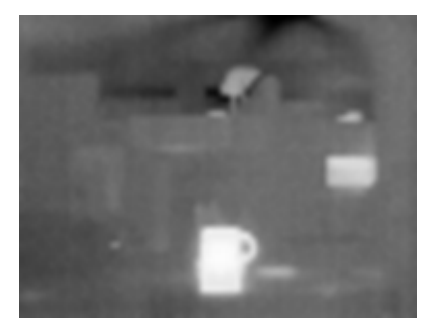
\includegraphics[width=.30\textwidth]{linearAGCc.png}}
    \caption{Comparison of Linear AGC and Classic/Lepton Variant of Histogram Equalization}
    \label{fig:comparisionlinearAGC}
\end{figure}
%
A high value of clip limit high results in a mapping more like classic histogram
equalization, whereas a low value results in mapping more like linear AGC. For
clip limit low, the opposite is true: a high value results in a mapping more
like linear AGC, whereas a low value results in a mapping more like classic
histogram equalization. The default values of both parameters produce a good
compromise between the two; however, because optimum AGC is highly subjective
and often application dependent, customers are encouraged to experiment to find
settings most appropriate for the target application. By default, the histogram
used to generate Lepton's 14-bit to 8-bit mapping function is collected from the
full array. In some applications, it is desirable to have the AGC algorithm
ignore a portion of the scene when collecting the histogram. For example, in
some applications it may be beneficial to optimize the display to a region of
interest (ROI) in the central portion of the image. When the AGC ROI is set to a
subset of the full image, any scene content located outside of the ROI is not
included in the histogram and therefore does not affect the mapping function
(note: this does not mean the portion outside of the ROI is not displayed or
that AGC is not applied there, only that those portions outside the AGC ROI do
not influence the mapping function).\cite{flirdatasheet}
%
